% !TEX root = ../main.tex
\chapter{Розрахунок оптимальних параметрів ПІ-регулятора і 
періоду квантування резонансним методом}\label{ch:resonance}
За завданням, розрахунки треба провести для об'єктів з передаточними функціями
$W_O(s) = \frac{
    k e^{-\tau s}
}{
    (T_1 s + 1) (T_2 s + 1) (T_3 s + 1)
}$ \eqref{W_0} та
$
W_{O_2}(s) = \frac{k e^{-\tau s}}{(T_1 s + 1)(T_2 s + 1)}
$ \eqref{W_02}.

Регулятор цифрового керування реалізує пропорційно-інтегральний закон керування, який представлений позиційним алгоритмом:
\begin{gather*}
    u(n T_0) = K_p \left(
        e(n T_0) + \frac{T_0}{T_I} \sum_{i=1}^n e(i T_0)
    \right)
\end{gather*}
Для визначення оптимальних параметрів настройки $K_{p_{\text{опт}}}$, $T_{I_{\text{опт}}}$ та періоду квантування
$T_{0_{\text{опт}}}$ скористаємося алгоритмом, наведеним у методичних рекомендаціях до курсової роботи.

\section{Випадок \texorpdfstring{$W_O(s) = \frac{
    k e^{-\tau s}
}{
    (T_1 s + 1) (T_2 s + 1) (T_3 s + 1)
}$}{1}}\label{sec:resonance_3rd_order}
а)\;  Шляхом розв'язання відносно частоти $\omega$ нелінійного рівняння
\begin{gather}
    \arctg{\omega T_1} + \arctg{\omega T_2} + \arctg{\omega T_3} + \omega \tau = 2.62
\end{gather}
знаходимо резонансну частоту $\omega_{\varphi_H} = 0.04096$ для неперервного контура керування.

б)\;  Визначаємо верхню та нижню частоту відносно резонансної частоти неперервної системи:
$\omega_{\varphi_H}^H = \frac{\omega_{\varphi_H}}{\sqrt{2}} = 0.02897$, 
$\omega_{\varphi_H}^B = {\sqrt{2}}{\omega_{\varphi_H}} = 0.05793$.

в)\; Використовуючи знайдену частоту $\omega_{\varphi_H}$, за формулою
\begin{gather}
    A(\omega) = \frac{k}{\sqrt{\left(1+\omega^2 T_1^2\right)\left(1+\omega^2 T_2^2\right)\left(1+\omega^2 T_3^2\right)}}
\end{gather}
знаходимо другий основний динамічний параметр неперервного контура в частотній області:
$A_H\left(\omega_{\varphi_H}\right) = 3.83604$. Також, знайдемо третій основний параметр
$\Phi_H(A) = \frac{A\left(\omega_{\varphi_H}^B\right)}{A\left(\omega_{\varphi_H}^H\right)} = 0.42790$.

г)\; Використовуючи вираз 
\begin{gather}
    \varphi(\omega) = \arctg{\omega T_1} + \arctg{\omega T_2} + \arctg{\omega T_3} + \omega \tau
\end{gather}
визначаємо четвертий основний параметр в частотній області для неперервного контуру:
$\Phi_H(\varphi) = \varphi\left(\omega_{\varphi_H}^H\right) - \varphi\left(\omega_{\varphi_H}^B\right) = 1.31497$.

д)\; За емпіричними формулами визначаємо оптимальні коефіцієнти настройки неперервного ПІ-регулятора
та оптимальний період квантування:
\begin{gather}
    T_{I_{\text{опт}}}^{\text{неп}} = 
    \frac{4.061 \cdot \Phi_H(A)^{-0.3387} \cdot \Phi_H(\varphi)^{0.2075}}{\omega_{\varphi_H}} \\
    K_{p_{\text{опт}}}^{\text{неп}} = \frac{1}{2 A_H\left(\omega_{\varphi_H}\right)}
    \cdot \left(
        1 + 1.189 \cdot \Phi_H(A)^{0.7139}\cdot \left(1.852 - \Phi_H(\varphi)\right)^{0.8643}
    \right) \\
    T_{0_{\text{опт}}} = \frac{
        0.5742 \cdot \Phi_H(A)^{0.5742} \Phi_H(\varphi)^{0.9394}
    }{\omega_{\varphi_H}}
\end{gather}
Отримуємо значення
$T_{I_{\text{опт}}}^{\text{неп}} = 139.88408$, $K_{p_{\text{опт}}}^{\text{неп}} = 0.17974$,
$T_{0_{\text{опт}}} = 11.13496$.

е)\; При оптимальному періоду квантування визначаємо чотири основні параметри 
$\omega_{\varphi}$, $A\left(\omega_{\varphi}\right)$, $\Phi(A)$, $\Phi(\varphi)$
в частотній області при врахуванні ПНЧ об'єкта. Для цього використаємо рівняння
\begin{gather}\label{A_w_1}
    A(\omega) = A_H(\omega) \cdot \frac{
        \sin {\frac{\omega T_{0_{\text{опт}}}}{2}}
    }{
        {\frac{\omega T_{0_{\text{опт}}}}{2}}
    } \\ \label{phi_w_1}
    \varphi(\omega) = 
    \arctg{\omega T_1} + \arctg{\omega T_2} + \arctg{\omega T_3} + \omega \tau + {\frac{\omega T_{0_{\text{опт}}}}{2}}
\end{gather}
Шляхом розв'язання $\varphi(\omega) = 2.62$ знаходимо частоту 
$\omega_{\varphi} = 0.03670$, а потім за рівняннями \eqref{A_w_1}, \eqref{phi_w_1} знаходимо 
$A\left(\omega_{\varphi}\right) = 4.32464$, 
$\Phi(A) = \frac{A\left(\omega_{\varphi_H}^B\right)}{A\left(\omega_{\varphi_H}^H\right)} = 0.46223$, 
$\Phi(\varphi) = \varphi\left(\omega_{\varphi_H}^H\right) - \varphi\left(\omega_{\varphi_H}^B\right) = 1.39902$.

ж)\; При оптимальному періоді квантування $T_{0_{\text{опт}}}$ знаходимо 
оптимальні значення $T_{I_{\text{опт}}}$ та $K_{p_{\text{опт}}}$ за формулами
\begin{gather}
    T_{I_{\text{опт}}} = 
    \frac{4.061 \cdot \Phi(A)^{-0.3387} \cdot \Phi(\varphi)^{0.2075}}{\omega_{\varphi}} \\
    K_{p_{\text{опт}}} = \frac{1}{2 A\left(\omega_{\varphi_H}\right)}
    \cdot \left(
        1 + 1.189 \cdot \Phi(A)^{0.7139}\cdot \left(1.852 - \Phi(\varphi)\right)^{0.8843}
    \right)
\end{gather}
Отримуємо значення
$T_{I_{\text{опт}}} = 154.07932$, $K_{p_{\text{опт}}} = 0.15558$.

Зберемо результати обчислень до таблиці:
\begin{center}
    \begin{tabular}{|c|c|}
        \hline
        параметр & значення \\
        \hline
        $\omega_{\varphi_H}$ & 0.04096\\
        \hline
        $\omega_{\varphi_H}^H$ & 0.02897\\
        \hline
        $\omega_{\varphi_H}^BH$ & 0.05793\\
        \hline
        $A_H\left(\omega_{\varphi_H}\right)$ & 3.83604\\
        \hline
        $\Phi_H(A)$ & 0.42790\\
        \hline
        $\Phi_H(\varphi)$ & 1.31497\\
        \hline
        $T_{I_{\text{опт}}}^{\text{неп}}$ & 139.88408\\
        \hline
        $K_{p_{\text{опт}}}^{\text{неп}}$ & 0.17974\\
        \hline
        $T_{0_{\text{опт}}}$ & 11.13496\\
        \hline
        $\omega_{\varphi}$ & 0.03670\\
        \hline
        $A\left(\omega_{\varphi}\right)$ & 4.32464\\
        \hline
        $\Phi(A)$ & 0.46223\\
        \hline
        $\Phi(\varphi)$ & 1.39902\\
        \hline
        $T_{I_{\text{опт}}}$ & 154.07932\\
        \hline
        $K_{p_{\text{опт}}}$ & 0.15495\\
        \hline
     \end{tabular}
\end{center}
Для цифрового моделювання перехідного процесу вихідної координати $y$ скористаємося передаточною функцією $W_\text{з}(s)$:
\begin{gather*}
    \mbox{\normalsize $y(s) = W_\text{з}(s) G(s) = \frac{W_p(s) W_O(s)}{1 + W_p(s) W_O(s)} G(s)$} \\
    \mbox{\normalsize $W_p(s) = K_{p_{\text{опт}}} \left(1 + \frac{1}{T_{I_{\text{опт}}} s}\right), \;
    G(s) = \frac{1}{s} \left(1 - e^{-s T_{0_{\text{опт}}}}\right)$}
\end{gather*}

Чисельно знайшовши обернене перетворення Лапласа від $y(s)$ в моменти $n T_{0_{\text{опт}}}$, 
отримаємо значення вихідної координати при подачі на задаюче діяння одиничного імпульсу довжиною $T_{0_{\text{опт}}}$. 
Відношення затухання дорівнює $\frac{B}{A} = \frac{0.29424}{0.04990} = 0.16958$.
\begin{center}
    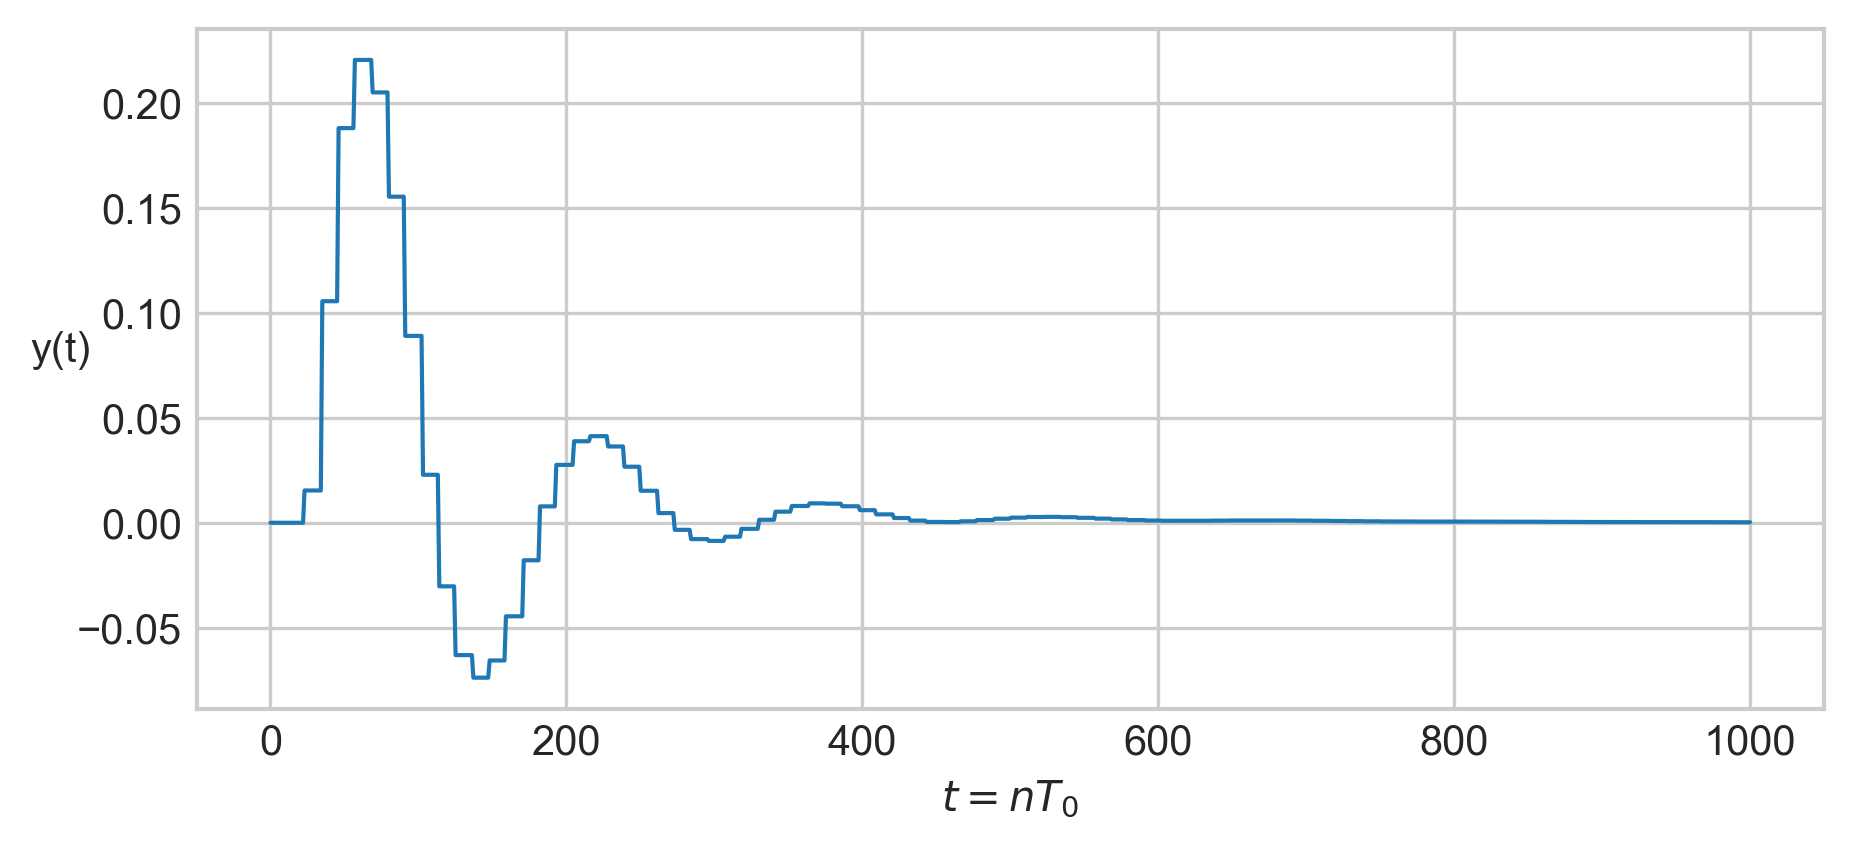
\includegraphics[scale=0.9]{pics/transient_process_task_5_1.png}
\end{center}

\section{Випадок \texorpdfstring{$W_{O_2}(s) = \frac{k e^{-\tau s}}{(T_1 s + 1)(T_2 s + 1)}$}{2}}
\label{sec:resonance_2nd_order}
а)\;  Шляхом розв'язання відносно частоти $\omega$ нелінійного рівняння
\begin{gather}
    \arctg{\omega T_1} + \arctg{\omega T_2} + \omega \tau = 2.62
\end{gather}
знаходимо резонансну частоту $\omega_{\varphi_H} = 0.05341$ для неперервного контура керування.

б)\;  Визначаємо верхню та нижню частоту відносно резонансної частоти неперервної системи:
$\omega_{\varphi_H}^H = \frac{\omega_{\varphi_H}}{\sqrt{2}} = 0.03777$, 
$\omega_{\varphi_H}^B = {\sqrt{2}}{\omega_{\varphi_H}} = 0.07553$.

в)\; Використовуючи знайдену частоту $\omega_{\varphi_H}$, за формулою
\begin{gather}
    A(\omega) = \frac{k}{\sqrt{\left(1+\omega^2 T_1^2\right)\left(1+\omega^2 T_2^2\right)\left(1+\omega^2 T_3^2\right)}}
\end{gather}
знаходимо другий основний динамічний параметр неперервного контура в частотній області:
$A_H\left(\omega_{\varphi_H}\right) = 3.08583$. Також, знайдемо третій основний параметр
$\Phi_H(A) = \frac{A\left(\omega_{\varphi_H}^B\right)}{A\left(\omega_{\varphi_H}^H\right)} = 0.41264$.

г)\; Використовуючи вираз 
\begin{gather}
    \varphi(\omega) = \arctg{\omega T_1} + \arctg{\omega T_2} + \arctg{\omega T_3} + \omega \tau
\end{gather}
визначаємо четвертий основний параметр в частотній області для неперервного контуру:
$\Phi_H(\varphi) = \varphi\left(\omega_{\varphi_H}^H\right) - \varphi\left(\omega_{\varphi_H}^B\right) = 1.15456$.

д)\; За емпіричними формулами визначаємо оптимальні коефіцієнти настройки неперервного ПІ-регулятора
та оптимальний період квантування:
\begin{gather}
    T_{I_{\text{опт}}}^{\text{неп}} = 
    \frac{4.061 \cdot \Phi_H(A)^{-0.3387} \cdot \Phi_H(\varphi)^{0.2075}}{\omega_{\varphi_H}} \\
    K_{p_{\text{опт}}}^{\text{неп}} = \frac{1}{2 A_H\left(\omega_{\varphi_H}\right)}
    \cdot \left(
        1 + 1.189 \cdot \Phi_H(A)^{0.7139}\cdot \left(1.852 - \Phi_H(\varphi)\right)^{0.8643}
    \right) \\
    T_{0_{\text{опт}}} = \frac{
        0.5742 \cdot \Phi_H(A)^{0.5742} \Phi_H(\varphi)^{0.9394}
    }{\omega_{\varphi_H}}
\end{gather}
Отримуємо значення
$T_{I_{\text{опт}}}^{\text{неп}} = 105.72649$, $K_{p_{\text{опт}}}^{\text{неп}} = 0.23703$,
$T_{0_{\text{опт}}} = 7.40205$.

е)\; При оптимальному періоду квантування визначаємо чотири основні параметри 
$\omega_{\varphi}$, $A\left(\omega_{\varphi}\right)$, $\Phi(A)$, $\Phi(\varphi)$
в частотній області при врахуванні ПНЧ об'єкта. Для цього використаємо рівняння
\begin{gather}\label{A_w_2}
    A(\omega) = A_H(\omega) \cdot \frac{
        \sin {\frac{\omega T_{0_{\text{опт}}}}{2}}
    }{
        {\frac{\omega T_{0_{\text{опт}}}}{2}}
    } \\ \label{phi_w_2}
    \varphi(\omega) = 
    \arctg{\omega T_1} + \arctg{\omega T_2} + \arctg{\omega T_3} + \omega \tau + {\frac{\omega T_{0_{\text{опт}}}}{2}}
\end{gather}
Шляхом розв'язання $\varphi(\omega) = 2.62$ знаходимо частоту 
$\omega_{\varphi} = 0.04792$, а потім за рівняннями \eqref{A_w_1}, \eqref{phi_w_1} знаходимо 
$A\left(\omega_{\varphi}\right) = 3.51065$, 
$\Phi(A) = \frac{A\left(\omega_{\varphi_H}^B\right)}{A\left(\omega_{\varphi_H}^H\right)} = 0.43618$, 
$\Phi(\varphi) = \varphi\left(\omega_{\varphi_H}^H\right) - \varphi\left(\omega_{\varphi_H}^B\right) = 1.23981$.

ж)\; При оптимальному періоді квантування $T_{0_{\text{опт}}}$ знаходимо 
оптимальні значення $T_{I_{\text{опт}}}$ та $K_{p_{\text{опт}}}$ за формулами
\begin{gather}
    T_{I_{\text{опт}}} = 
    \frac{4.061 \cdot \Phi(A)^{-0.3387} \cdot \Phi(\varphi)^{0.2075}}{\omega_{\varphi}} \\
    K_{p_{\text{опт}}} = \frac{1}{2 A\left(\omega_{\varphi_H}\right)}
    \cdot \left(
        1 + 1.189 \cdot \Phi(A)^{0.7139}\cdot \left(1.852 - \Phi(\varphi)\right)^{0.8843}
    \right)
\end{gather}
Отримуємо значення
$T_{I_{\text{опт}}} = 117.36092$, $K_{p_{\text{опт}}} = 0.20311$.

Зберемо результати обчислень до таблиці:
\begin{center}
    \begin{tabular}{|c|c|}
        \hline
        параметр & значення \\
        \hline
        $\omega_{\varphi_H}$ & 0.05341\\
        \hline
        $\omega_{\varphi_H}^H$ & 0.03777\\
        \hline
        $\omega_{\varphi_H}^BH$ & 0.07553\\
        \hline
        $A_H\left(\omega_{\varphi_H}\right)$ & 3.08583\\
        \hline
        $\Phi_H(A)$ & 0.41264\\
        \hline
        $\Phi_H(\varphi)$ & 1.15456\\
        \hline
        $T_{I_{\text{опт}}}^{\text{неп}}$ & 105.72649\\
        \hline
        $K_{p_{\text{опт}}}^{\text{неп}}$ & 0.23703\\
        \hline
        $T_{0_{\text{опт}}}$ & 7.40205\\
        \hline
        $\omega_{\varphi}$ & 0.04792\\
        \hline
        $A\left(\omega_{\varphi}\right)$ & 3.51065\\
        \hline
        $\Phi(A)$ & 0.43618\\
        \hline
        $\Phi(\varphi)$ & 1.23981\\
        \hline
        $T_{I_{\text{опт}}}$ & 117.36092\\
        \hline
        $K_{p_{\text{опт}}}$ & 0.20311\\
        \hline
     \end{tabular}
\end{center}

Цифрове моделювання перехідного процесу вихідної координати $y$ проведемо аналогічно попередньому пункту. 
Відношення затухання дорівнює 
$\frac{B}{A} = \frac{0.28438}{0.04621} = 0.16249$.
\begin{center}
    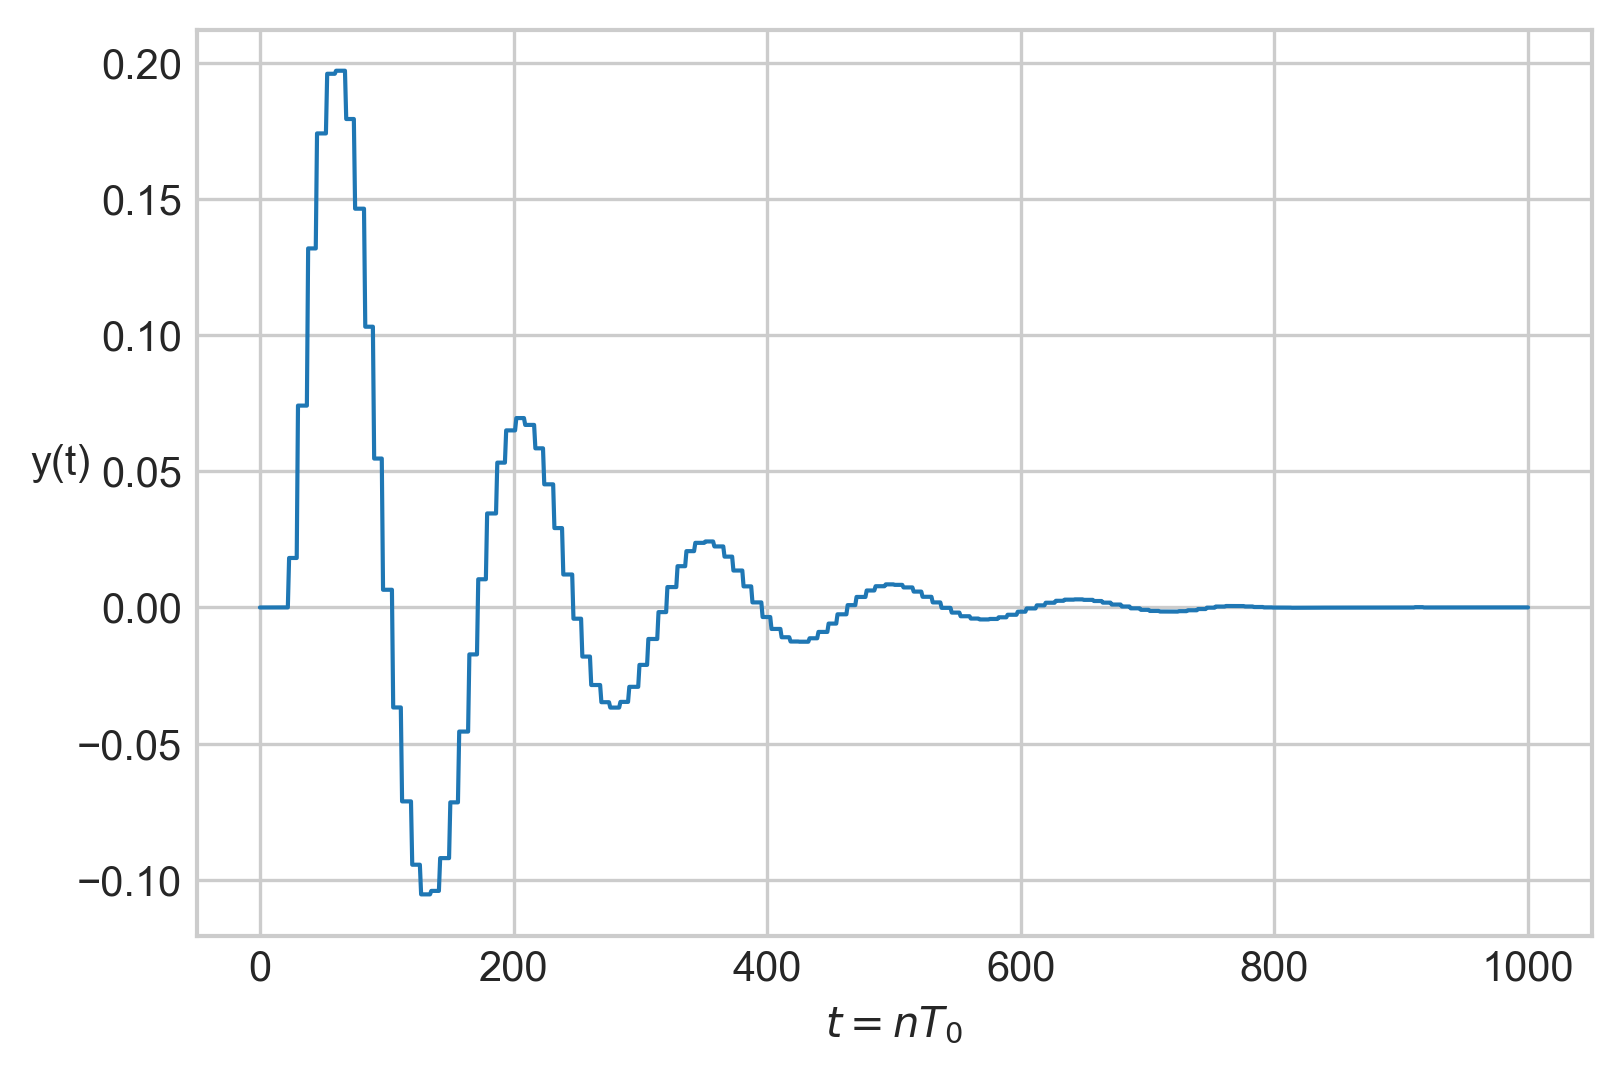
\includegraphics[scale=0.9]{pics/transient_process_task_5_2.png}
\end{center}